% Options for packages loaded elsewhere
\PassOptionsToPackage{unicode}{hyperref}
\PassOptionsToPackage{hyphens}{url}
\PassOptionsToPackage{dvipsnames,svgnames,x11names}{xcolor}
%
\documentclass[
  12pt,
  letterpaper,
  DIV=11,
  numbers=noendperiod]{scrartcl}

\usepackage{amsmath,amssymb}
\usepackage{setspace}
\usepackage{iftex}
\ifPDFTeX
  \usepackage[T1]{fontenc}
  \usepackage[utf8]{inputenc}
  \usepackage{textcomp} % provide euro and other symbols
\else % if luatex or xetex
  \usepackage{unicode-math}
  \defaultfontfeatures{Scale=MatchLowercase}
  \defaultfontfeatures[\rmfamily]{Ligatures=TeX,Scale=1}
\fi
\usepackage{lmodern}
\ifPDFTeX\else  
    % xetex/luatex font selection
    \setmainfont[]{Palatino}
  \setmathfont[]{STIX Two Math}
\fi
% Use upquote if available, for straight quotes in verbatim environments
\IfFileExists{upquote.sty}{\usepackage{upquote}}{}
\IfFileExists{microtype.sty}{% use microtype if available
  \usepackage[]{microtype}
  \UseMicrotypeSet[protrusion]{basicmath} % disable protrusion for tt fonts
}{}
\makeatletter
\@ifundefined{KOMAClassName}{% if non-KOMA class
  \IfFileExists{parskip.sty}{%
    \usepackage{parskip}
  }{% else
    \setlength{\parindent}{0pt}
    \setlength{\parskip}{6pt plus 2pt minus 1pt}}
}{% if KOMA class
  \KOMAoptions{parskip=half}}
\makeatother
\usepackage{xcolor}
\usepackage[margin=1in]{geometry}
\setlength{\emergencystretch}{3em} % prevent overfull lines
\setcounter{secnumdepth}{5}
% Make \paragraph and \subparagraph free-standing
\makeatletter
\ifx\paragraph\undefined\else
  \let\oldparagraph\paragraph
  \renewcommand{\paragraph}{
    \@ifstar
      \xxxParagraphStar
      \xxxParagraphNoStar
  }
  \newcommand{\xxxParagraphStar}[1]{\oldparagraph*{#1}\mbox{}}
  \newcommand{\xxxParagraphNoStar}[1]{\oldparagraph{#1}\mbox{}}
\fi
\ifx\subparagraph\undefined\else
  \let\oldsubparagraph\subparagraph
  \renewcommand{\subparagraph}{
    \@ifstar
      \xxxSubParagraphStar
      \xxxSubParagraphNoStar
  }
  \newcommand{\xxxSubParagraphStar}[1]{\oldsubparagraph*{#1}\mbox{}}
  \newcommand{\xxxSubParagraphNoStar}[1]{\oldsubparagraph{#1}\mbox{}}
\fi
\makeatother


\providecommand{\tightlist}{%
  \setlength{\itemsep}{0pt}\setlength{\parskip}{0pt}}\usepackage{longtable,booktabs,array}
\usepackage{calc} % for calculating minipage widths
% Correct order of tables after \paragraph or \subparagraph
\usepackage{etoolbox}
\makeatletter
\patchcmd\longtable{\par}{\if@noskipsec\mbox{}\fi\par}{}{}
\makeatother
% Allow footnotes in longtable head/foot
\IfFileExists{footnotehyper.sty}{\usepackage{footnotehyper}}{\usepackage{footnote}}
\makesavenoteenv{longtable}
\usepackage{graphicx}
\makeatletter
\newsavebox\pandoc@box
\newcommand*\pandocbounded[1]{% scales image to fit in text height/width
  \sbox\pandoc@box{#1}%
  \Gscale@div\@tempa{\textheight}{\dimexpr\ht\pandoc@box+\dp\pandoc@box\relax}%
  \Gscale@div\@tempb{\linewidth}{\wd\pandoc@box}%
  \ifdim\@tempb\p@<\@tempa\p@\let\@tempa\@tempb\fi% select the smaller of both
  \ifdim\@tempa\p@<\p@\scalebox{\@tempa}{\usebox\pandoc@box}%
  \else\usebox{\pandoc@box}%
  \fi%
}
% Set default figure placement to htbp
\def\fps@figure{htbp}
\makeatother
% definitions for citeproc citations
\NewDocumentCommand\citeproctext{}{}
\NewDocumentCommand\citeproc{mm}{%
  \begingroup\def\citeproctext{#2}\cite{#1}\endgroup}
\makeatletter
 % allow citations to break across lines
 \let\@cite@ofmt\@firstofone
 % avoid brackets around text for \cite:
 \def\@biblabel#1{}
 \def\@cite#1#2{{#1\if@tempswa , #2\fi}}
\makeatother
\newlength{\cslhangindent}
\setlength{\cslhangindent}{1.5em}
\newlength{\csllabelwidth}
\setlength{\csllabelwidth}{3em}
\newenvironment{CSLReferences}[2] % #1 hanging-indent, #2 entry-spacing
 {\begin{list}{}{%
  \setlength{\itemindent}{0pt}
  \setlength{\leftmargin}{0pt}
  \setlength{\parsep}{0pt}
  % turn on hanging indent if param 1 is 1
  \ifodd #1
   \setlength{\leftmargin}{\cslhangindent}
   \setlength{\itemindent}{-1\cslhangindent}
  \fi
  % set entry spacing
  \setlength{\itemsep}{#2\baselineskip}}}
 {\end{list}}
\usepackage{calc}
\newcommand{\CSLBlock}[1]{\hfill\break\parbox[t]{\linewidth}{\strut\ignorespaces#1\strut}}
\newcommand{\CSLLeftMargin}[1]{\parbox[t]{\csllabelwidth}{\strut#1\strut}}
\newcommand{\CSLRightInline}[1]{\parbox[t]{\linewidth - \csllabelwidth}{\strut#1\strut}}
\newcommand{\CSLIndent}[1]{\hspace{\cslhangindent}#1}

\widowpenalty=10000
\clubpenalty=10000
\setlength{\parindent}{2.4em}
\setlength{\parskip}{0em}
\usepackage{indentfirst}
\usepackage{mathtools, nccmath}
\usepackage[page,header]{appendix}
\usepackage{titletoc}
\usepackage[labelfont=bf]{caption}
\usepackage{lscape}
\usepackage{setspace}
\newcommand{\blandscape}{\begin{landscape}}
\newcommand{\elandscape}{\end{landscape}}
\newcommand{\bcen}{\begin{center}}
\newcommand{\ecen}{\end{center}}
\newcommand{\tsp}{\thinspace}
\pagenumbering{arabic}
\footskip 0.5in
\usepackage{titlesec}
\titlespacing\section{0pt}{6pt}{0pt}
\titlespacing\subsection{0pt}{10pt}{0pt}
\titlespacing\subsubsection{0pt}{10pt}{0pt}
\titleformat{\section}{\large\bfseries}{\thesection.}{.75em}{}
\titleformat{\subsection}{\normalsize\bfseries}{\thesubsection.}{.75em}{}
\titleformat{\subsubsection}{\normalsize\bfseries\itshape}{\thesubsubsection.}{.75em}{}


\KOMAoption{captions}{tableheading}
\makeatletter
\@ifpackageloaded{caption}{}{\usepackage{caption}}
\AtBeginDocument{%
\ifdefined\contentsname
  \renewcommand*\contentsname{Table of contents}
\else
  \newcommand\contentsname{Table of contents}
\fi
\ifdefined\listfigurename
  \renewcommand*\listfigurename{List of Figures}
\else
  \newcommand\listfigurename{List of Figures}
\fi
\ifdefined\listtablename
  \renewcommand*\listtablename{List of Tables}
\else
  \newcommand\listtablename{List of Tables}
\fi
\ifdefined\figurename
  \renewcommand*\figurename{Figure}
\else
  \newcommand\figurename{Figure}
\fi
\ifdefined\tablename
  \renewcommand*\tablename{Table}
\else
  \newcommand\tablename{Table}
\fi
}
\@ifpackageloaded{float}{}{\usepackage{float}}
\floatstyle{ruled}
\@ifundefined{c@chapter}{\newfloat{codelisting}{h}{lop}}{\newfloat{codelisting}{h}{lop}[chapter]}
\floatname{codelisting}{Listing}
\newcommand*\listoflistings{\listof{codelisting}{List of Listings}}
\makeatother
\makeatletter
\makeatother
\makeatletter
\@ifpackageloaded{caption}{}{\usepackage{caption}}
\@ifpackageloaded{subcaption}{}{\usepackage{subcaption}}
\makeatother

\usepackage{bookmark}

\IfFileExists{xurl.sty}{\usepackage{xurl}}{} % add URL line breaks if available
\urlstyle{same} % disable monospaced font for URLs
\hypersetup{
  pdftitle={Comparing Encoder-Based Models for Event Coding},
  pdfauthor={Emmanuel Teitelbaum; Mohiddin Bacha Shaik; Shiva Chakrabarty Sharma},
  colorlinks=true,
  linkcolor={Blue4},
  filecolor={Maroon},
  citecolor={Blue},
  urlcolor={Blue},
  pdfcreator={LaTeX via pandoc}}


\title{Comparing Encoder-Based Models for Event Coding\footnote{Prepared
  for the Advancing the Use of Computational Tools in Political Science
  Virtual Research Group, held under the auspices of the 2025 American
  Political Science Virtual Research Meetings. The authors would like to
  thank Aravind Chinnari for his help with earlier versions of the
  models presented in this paper. Our code and data can be accessed at
  https://github.com/eteitelbaum/code-satp.}}
\usepackage{etoolbox}
\makeatletter
\providecommand{\subtitle}[1]{% add subtitle to \maketitle
  \apptocmd{\@title}{\par {\large #1 \par}}{}{}
}
\makeatother
\subtitle{Evidence from the South Asia Terrorism Portal}
\author{Emmanuel Teitelbaum\footnote{George Washington University,
  Department of Political Science} \and Mohiddin Bacha
Shaik\footnote{George Washington University, Data Science Program} \and Shiva
Chakrabarty Sharma\footnote{George Washington University, Trachtenberg
  School of Public Policy}}
\date{April 7, 2025}

\begin{document}
\maketitle
\begin{abstract}
\vspace{4em}

\noindent

\begin{center}
\textit{Early draft. Do not circulate.} \\
\vspace{4em}
\textbf{Word count}: 3,710
\end{center}
\newpage{}
\begin{center}
\textbf{ABSTRACT}
\end{center}
\vspace{1em}

\noindent \normalsize This paper compares the performance of
encoder-based transformer models on a series of conflict-related coding
tasks. Using hand-coded data from the South Asia Terrorism Portal (SATP)
pertaining to the Maoist insurgency in India, we evaluate six
models---BERT, RoBERTa, ELECTRA, DistilBERT, XLNet, and the
domain-specific ConfliBERT---across multiple dimensions. Events are
annotated with overlapping labels capturing forms of violence and state
response, allowing us to assess model performance across label
frequency, lexical complexity, and training data availability. We also
evaluate inference speed to reflect practical constraints in
low-resource academic settings. While ConfliBERT performs well overall,
particularly on rare and semantically nuanced labels, RoBERTa matches
its accuracy on many tasks and runs at comparable speed. All models
perform strongly on frequent, lexically distinctive labels but struggle
with rare or adjacent categories. These results highlight the promise of
general-purpose open-source models for many annotation tasks, the modest
gains from domain-specific pretraining, and the persistent challenges of
rare label prediction. We conclude with recommendations for improving
classification performance on difficult categories and discuss the
broader tradeoffs between model complexity, annotation cost, and
workflow design in applied conflict research. \newpage
\end{abstract}


\setstretch{2}
\section{Introduction}\label{introduction}

Large language models (LLMs) are rapidly changing how political
scientists and conflict researchers analyze unstructured text.
Transformer-based architectures now dominate natural language processing
(NLP), offering improved performance over traditional methods such as
bag-of-words models, dictionaries, and supervised classifiers. These
advances have generated enthusiasm for the possibility that LLMs might
dramatically reduce the labor involved in annotating political texts,
particularly for tasks like sentiment classification, ideology scaling,
and structured event coding.

In political science, early evaluations of general-purpose models such
as GPT-3 and GPT-4 demonstrated strong performance on relatively
straightforward tasks, especially in English and on short texts. For
example, Heseltine and Clemm von Hohenberg
(\citeproc{ref-heseltine2024}{2024}) show that GPT-4 achieves high
accuracy on sentiment and political relevance classification across
multiple countries, while Ornstein, Blasingame, and Truscott
(\citeproc{ref-ornstein2023}{2023}) find that GPT-3 can match or exceed
human coding across several political applications. These studies helped
establish the feasibility of LLM-assisted annotation, particularly for
binary or categorical tasks involving relatively unambiguous inputs.

Building on this foundation, researchers in conflict studies have begun
developing domain-specific models trained on political violence and
protest corpora. ConfliBERT (\citeproc{ref-hu2022}{Hu et al. 2022};
\citeproc{ref-brandt2024}{Brandt et al. 2024}) is the most prominent
example, a BERT-based model pre-trained on tens of gigabytes of
conflict-related text. It consistently outperforms general-purpose
models on event classification, actor extraction, and named entity
recognition. Similarly, Halterman et al.
(\citeproc{ref-halterman2023}{2023}) introduce NGEC, a modular
transformer-based pipeline for extracting structured political events,
emphasizing flexibility across coding ontologies and contexts.

These models have shifted the conversation from whether LLMs are viable
for political science to how best to deploy them. In particular,
domain-specific pretraining has been presented as a necessary step for
achieving state-of-the-art results in applied research. Yet this
assumption is often difficult to evaluate in practice, especially for
researchers working with constrained resources or seeking to reuse
existing open-access models. Moreover, many of the most time-consuming
tasks in political event coding---such as identifying common event types
or actor roles---are conceptually routine, even if they appear in
bespoke datasets.

This paper revisits the promise and limits of domain-specific LLMs in
the context of a series of conflict-related classification tasks. We use
a subset of event descriptions from the South Asia Terrorism Portal
(SATP), focusing on the Maoist insurgency in India. Events were
hand-coded by researchers using a multi-label taxonomy capturing event
type, actor behavior, and modalities of violence. The labels vary in
frequency and complexity, ranging from common, lexically distinctive
labels like \emph{killing} to more semantically ambiguous ones such as
\emph{infrastructure attack}. While the dataset shares many structural
features with other conflict datasets---such as GTD, ICEWS, or
Polecat---it also reflects includes some relatively niche labels that
were specific to the interests of the researchers working on this
specific project.

Our study makes several contributions. First, we evaluate and compare
several transformer-based models commonly used in political text
classification: BERT, DistilBERT, ELECTRA, RoBERTa, XLNet, and the
domain-specific ConfliBERT. We examine how model performance varies
across labels and training data fractions. Second, we incorporate
inference speed into our evaluation. This is an important consideration
in academic and low-resource environments where compute budgets are
constrained. We find that while ConfliBERT performs best overall,
RoBERTa matches its performance on many labels and runs at comparable
speed---complicating the argument that domain-specific pretraining is
always necessary for strong performance.

Third, we assess how models handle lexically complex and low-frequency
labels. These are often the very tasks that would be delegated to
graduate student coders or domain experts due to their ambiguity or
theoretical salience. Our results show that even well-trained models
struggle with such categories, and that performance gains are uneven
across the label space. While transformer-based models can reliably code
frequent and lexically grounded labels with minimal supervision, they
remain inconsistent on semantically adjacent or underrepresented
categories.

In short, our findings suggest that open-source general-purpose models
can be highly effective for a wide range of political coding tasks,
including many found in conflict datasets. Domain-specific models like
ConfliBERT provide additional accuracy, particularly when label
definitions are subtle or data are scarce, but their advantages may be
incremental rather than wholly transformative. For many
applications---particularly those involving routine coding tasks---open
models such as RoBERTa may offer a sufficient balance of speed,
accuracy, and accessibility.

The remainder of the paper proceeds as follows. We begin by describing
the dataset and coding framework. We then outline the modeling approach,
evaluation metrics, and experimental design. Results are presented with
attention to model comparisons, error patterns, and performance
variation by label type. We conclude with a discussion of implications
for future annotation strategies, especially in low-resource research
settings, and point to concrete paths for improving model performance on
rare and ambiguous labels.

\section{The SATP Maoist Violence Incidents
Dataset}\label{the-satp-maoist-violence-incidents-dataset}

The South Asia Terrorism Portal (SATP) is a foundational resource for
scholars of political violence in South Asia. Its curated event
summaries offer one of the most comprehensive, longitudinal collections
of open-source conflict data on the region, with particular relevance
for research on insurgency, terrorism, and counterinsurgency in India.
Recent work in political event classification using large language
models (LLMs) has employed SATP as a source of annotated conflict data
for supervised learning and model evaluation. Hu et al.
(\citeproc{ref-hu2022}{2022}) used the SATP dataset to test ConfliBERT,
a BERT-based model trained on a large corpus of political violence
texts, evaluating it on binary classification tasks like identifying
whether a report described a violent event and multi-label
classification like assigning event types such as armed assault or
bombing. Brandt et al. (\citeproc{ref-brandt2024}{2024}) extended this
work by comparing ConfliBERT to more recent decoder-based LLMs, using
SATP again for illustrative examples while shifting the primary
evaluation focus to larger-scale datasets such as the Global Terrorism
Database (GTD).

In our study, we draw on the same underlying SATP news reports to
construct a distinct dataset focused exclusively on violence associated
with the Maoist insurgency. Our dataset spans the years 2005 to 2016, a
period that overlaps with but also precedes the SATP-based annotations
used in the ConfliBERT studies. This timeframe was selected to align
with the peak intensity of Maoist activity in India. Like Hu et al., we
work at the level of incident summaries reported in SATP, but our coding
is tailored to a single conflict and employs a more detailed and
conflict-specific annotation framework. Our dataset includes
approximately 10,000 events and is designed to test whether
transformer-based models can effectively classify complex,
context-dependent event types grounded in a specific political and
geographic setting.

The dataset was constructed through a multi-year coding project
involving undergraduate coders trained in political science and South
Asian studies, working under the supervision of graduate researchers
with domain expertise. Coders relied on a detailed codebook, developed
and refined over time, and entered structured data for each incident
using a standardized digital form. Each report was carefully parsed to
determine whether it contained multiple events or described a single
compound incident. Every incident received a unique identifier encoding
the state, date, and event sequence for that day.

The coding schema includes a range of variables not commonly found in
automated datasets including the perpetrator (or action taker) and a
broad range of target and action types. Where information allowed,
coders also captured the organizational role of perpetrators (e.g.,
commander, cadre, or sympathizer), and made distinctions between
government and private infrastructure when coding targets. Action types
were disaggregated to distinguish, for example, between armed assaults
and seizures, or between facility attacks and bombings. These
distinctions reflect coding priorities informed by field knowledge and
scholarly interest in the heterogeneity of violence within a single
conflict.

The coding process was characterized by an emphasis on quality control.
To ensure consistency and reliability, coders underwent structured
onboarding, participated in supervised trial phases, and engaged in
regular review and adjudication sessions to resolve edge cases.
Overlapping assignments were used to assess and calibrate inter-coder
reliability. A significant share of the dataset was double-coded, with
discrepancies reviewed and resolved by senior coders. In cases where
coding standards evolved over time, previously coded events were
revisited during the quality assurance phase to harmonize labels and
ensure consistency across the full time series.

While ConfliBERT and related BERT-based models have shown promising
results on classification tasks involving relatively broad event
categories, our dataset presents a more varied and nuanced test of LLM
capabilities. By coding more finely grained distinctions within a single
conflict, we aim to assess how well pretrained models can handle the
complexity of political violence data when applied to bespoke annotation
schemes. This challenge reflects the reality that researchers working
with real-world conflict data often require models that can disaggregate
events in ways that reflect local variation, political context, and
shifting repertoires of violence. In the following section, we outline
the specific tasks we set out to evaluate and compare how our selected
models performed on them.

\section{Methods}\label{methods}

To evaluate how effectively pretrained language models can recover
structured political violence data from unstructured text, we
implemented a series of classification tasks using our hand-coded SATP
Maoist Violence Incidents Dataset. The tasks reflect key dimensions of
political violence---actor type, action type, and target type---each
operationalized as either multi-class or multi-label classification
problems.

We evaluate model performance on three supervised learning tasks:

\begin{itemize}
\tightlist
\item
  A multi-class classification task to identify the \emph{perpetrator}
  (or actor) involved in each incident (Maoist, Security, or Other).
\item
  A multi-label classification task to identify the \emph{actions}
  taken, with possible labels including Armed Assault, Bombing,
  Abduction, Seizure, Arrest, Surrender, and Facility/Infrastructure
  Attack.
\item
  A second multi-label classification task to identify \emph{targets} of
  an attack or other action, with categories including Security,
  Civilians, Officials, Government Infrastructure, Private Property,
  Mining Companies, NGOs, Other Groups, and Maoists.
\end{itemize}

These tasks are extractive in nature and require the model to recover
structured labels from unstructured incident summaries. For this reason,
we restrict our evaluation to encoder-only transformer models, which are
better suited to classification and token-level prediction than
decoder-only models like GPT-style architectures. Encoder models
generate bidirectional contextual embeddings that allow them to attend
to all parts of the input simultaneously, a key advantage in tasks that
require understanding and resolving multiple co-occurring elements.

We selected six models for evaluation, all freely available via the
Hugging Face Model Hub:

\begin{itemize}
\tightlist
\item
  \emph{BERT-base-cased} (\citeproc{ref-devlin2019}{Devlin et al.
  2019}): A 12-layer, 110M parameter model pretrained on BooksCorpus and
  Wikipedia. It serves as the baseline encoder model for classification
  tasks.
\item
  \emph{DistilBERT-base-cased} (\citeproc{ref-sanh2020}{Sanh et al.
  2020}): A 6-layer, 66M parameter distilled version of BERT that is
  faster and lighter, designed to reduce inference cost with minimal
  performance loss.
\item
  \emph{RoBERTa-base} (\citeproc{ref-liu2019}{Liu et al. 2019}): A
  12-layer, 125M parameter BERT variant trained with more data and no
  next sentence prediction, generally outperforming BERT on downstream
  tasks.
\item
  \emph{ELECTRA-base-discriminator} (\citeproc{ref-clark2020}{Clark et
  al. 2020}): A 12-layer, 110M parameter model that uses a more
  sample-efficient pretraining objective (replaced token detection)
  rather than masked language modeling.
\item
  \emph{XLNet-base-cased} (\citeproc{ref-yang2020}{Yang et al. 2020}): A
  12-layer, 110M parameter autoregressive model trained with
  permutation-based language modeling, capable of modeling bidirectional
  context while retaining autoregressive benefits.
\item
  \emph{ConfliBERT} (\citeproc{ref-hu2022}{Hu et al. 2022}): A BERT-base
  model pretrained on a corpus of political violence and
  conflict-related text. It is domain-specific and designed to improve
  performance on tasks involving political conflict data.
\end{itemize}

All six models fall into the ``base'' category (between 66--125M
parameters), making them feasible to run on commodity hardware,
including laptops and free or low-tier Google Colab environments. This
makes them particularly well suited for use in low-resource
settings---both in terms of computational infrastructure and access to
large labeled datasets. Their relative efficiency also allows for more
flexible experimentation, such as evaluating performance across multiple
training data fractions.

Each model was fine-tuned on a fixed training--validation--test split
drawn from the full dataset. Approximately 2,000 incident descriptions
were randomly selected and held out at the start: 1,000 for validation
and 1,000 for final testing. The remaining \textasciitilde8,000
incidents were used in the training loop, where we iteratively varied
the size of the training set across six fractions: \(1/32\), \(1/16\),
\(1/8\), \(1/4\), \(1/2\), and the full training set. Validation and
test sets remained fixed throughout, allowing consistent comparison of
performance across data fractions and model architectures. All models
were fine-tuned using their cased versions, based on the assumption that
capitalization conveys important semantic and contextual information in
this domain---particularly for identifying proper nouns, such as
location names, political figures, or militant organizations, which are
common in South Asia--specific reporting.

To evaluate model performance, we report weighted macro F1 scores for
the multi-class perpetrator classification task and micro F1 scores for
the two multi-label classification tasks (action type and target type).
These metrics were selected to account for class imbalance while
preserving interpretability and comparability across settings.
Additional performance metrics, including precision, recall, and
per-label F1 scores, will be provided in an online supplement.

\section{Results}\label{results}

\subsection{Perpetrator Task}\label{perpetrator-task}

The perpetrator task is a multi-class classification problem in which
models are trained to predict the actor type responsible for a given
incident, with classes including Maoist, Security, and Other. Figure 1a
displays the weighted macro F1 scores achieved by each model across
different training data fractions. Figure 1b focuses on a single
fraction (\(1/8\) of the training set), presenting 95\% confidence
intervals obtained via bootstrap resampling (5,000 iterations) to assess
statistical uncertainty around model estimates.

\begin{figure}[H]

{\centering \pandocbounded{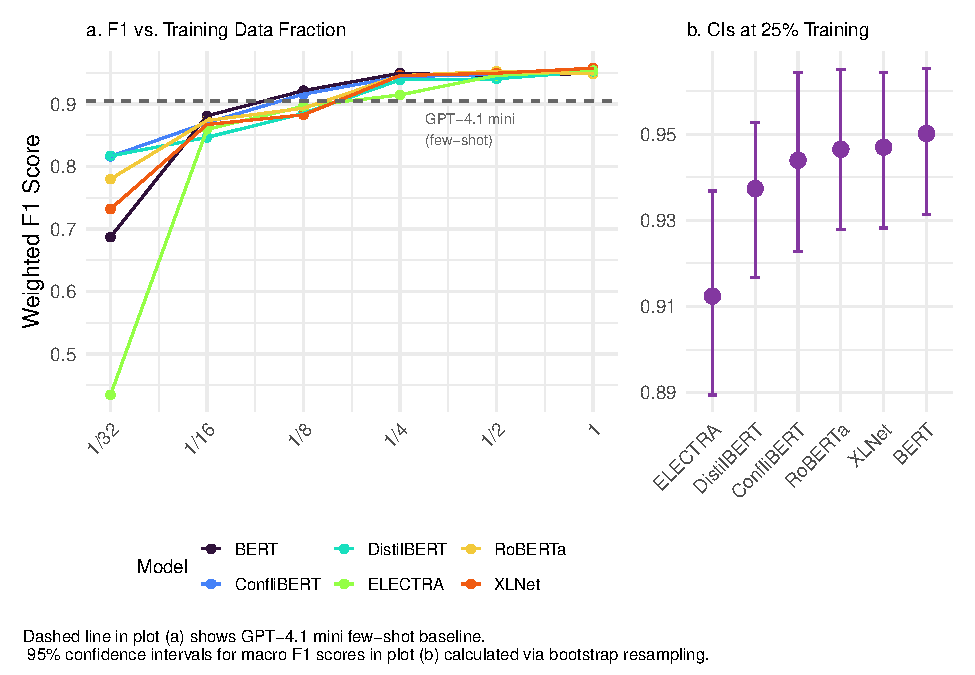
\includegraphics[keepaspectratio]{satp-classification_files/figure-pdf/perpetrator-1.pdf}}

}

\caption{Model Performance for `Perpetrator' Task}

\end{figure}%

Consistent with findings reported in the original ConfliBERT paper
(\citeproc{ref-hu2022}{Hu et al. 2022}), we observe that ConfliBERT
performs particularly well at lower data fractions, where its
domain-specific pretraining appears to confer an advantage. However, the
gap narrows quickly. At the 1/8 training level, RoBERTa and XLNet both
achieve F1 scores that are not statistically distinguishable from
ConfliBERT's, perhaps complicating a straightforward narrative about the
superiority of domain-specific model superiority
(\citeproc{ref-brandt2024}{Brandt et al. 2024};
\citeproc{ref-osorio2024}{Osorio et al. 2024}).

When trained on the full dataset, all models converge to very high
weighted macro F1 scores, ranging from 0.957 (ConfliBERT) to 0.968
(RoBERTa). This tight clustering in performance likely reflects the
relative simplicity of the classification task (predicting whether an
actor is Maoist, Security, or Other) and the benefit of high-quality,
consistent human annotations. While ConfliBERT retains a slight
advantage in low-resource settings, the results at full training suggest
that general-purpose encoder models are capable of matching or exceeding
the performance of domain-specific alternatives on this task. In a later
section, we return to inference speed and other performance trade-offs,
which further contextualize these results for applications in
low-resource environments.

\subsection{Action Type Task}\label{action-type-task}

The second task is a multi-label classification problem in which models
predict one or more action types associated with a given incident. These
include Armed Assault, Bombing, Abduction, Seizure, Arrest, Surrender,
and Facility/Infrastructure Attack. Performance is evaluated using micro
F1 scores, which are better suited to imbalanced, multi-label settings
where many samples carry multiple labels or none at all.

Figure 2a presents model performance across increasing training data
fractions. As in the perpetrator task, we observe notable variation in
learning rates. RoBERTa and XLNet clearly lead at the 25\% training
level (Figure 2b), with micro F1 scores of 0.882 and 0.879,
respectively. ConfliBERT trails modestly behind at 0.857, while BERT and
DistilBERT cluster around 0.800 and 0.785. ELECTRA performs
substantially worse, achieving a score of only 0.636 at this level.

\begin{figure}[H]

{\centering \pandocbounded{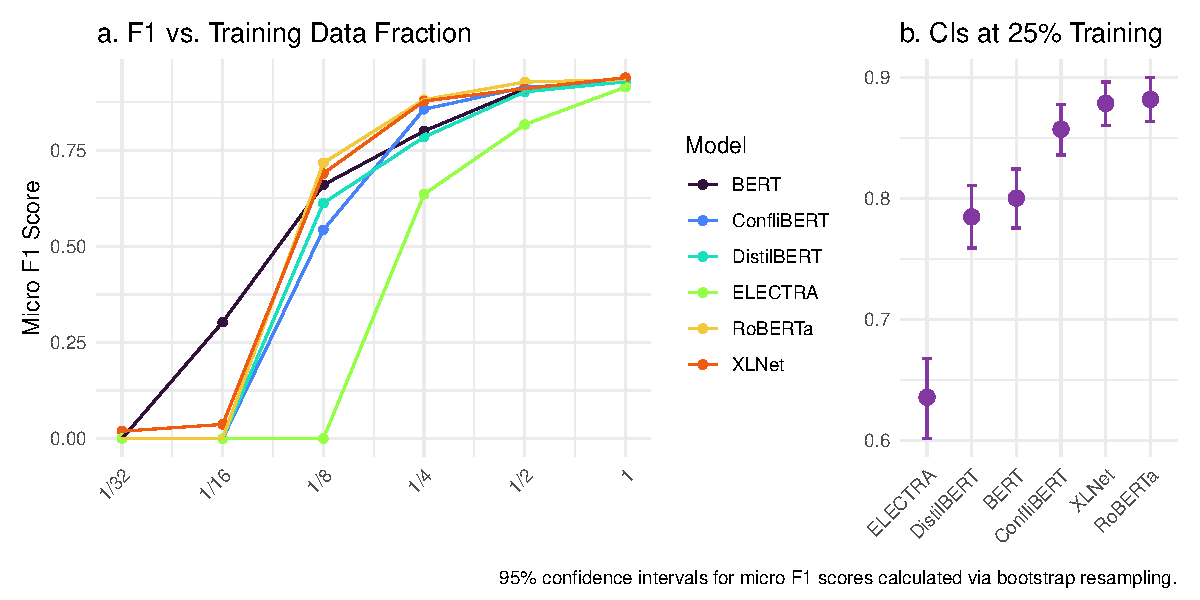
\includegraphics[keepaspectratio]{satp-classification_files/figure-pdf/action_type_performance-1.pdf}}

}

\caption{Model Performance for `Action Type' Task}

\end{figure}%

When trained on the full dataset, all models perform well, converging to
micro F1 scores in a narrow band between 0.915 (ELECTRA) and 0.939
(XLNet). The top four models---XLNet, RoBERTa, BERT, and
ConfliBERT---are separated by only a few hundredths of a point,
underscoring a high level of overall convergence. Once again, ConfliBERT
performs strongly in low-data regimes but is closely matched or
outperformed by general-purpose encoder models when more training data
are available.

\begin{figure}[H]

{\centering \pandocbounded{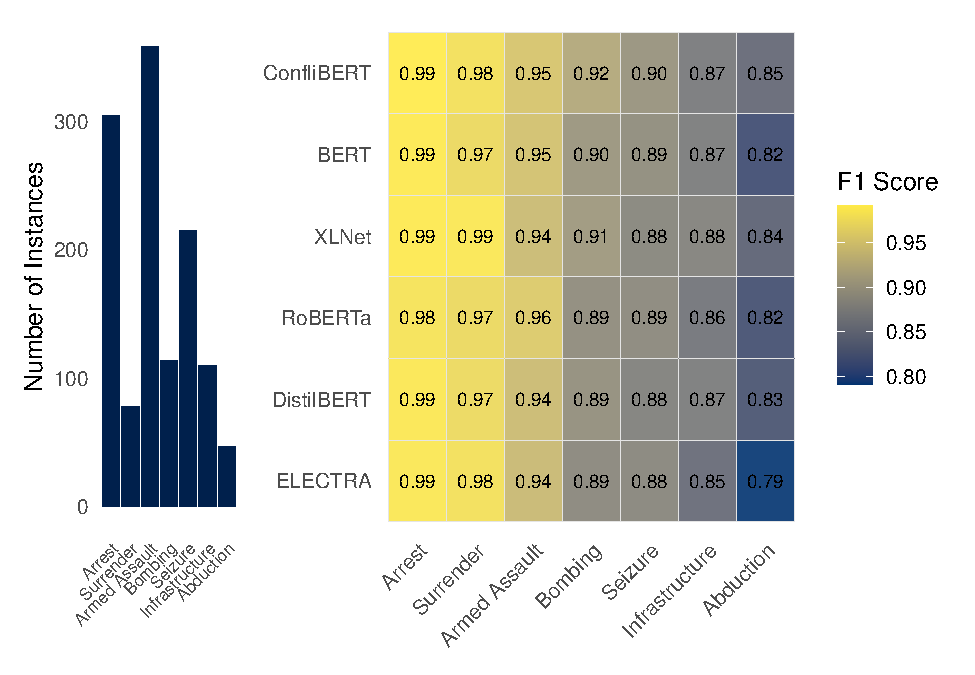
\includegraphics[keepaspectratio]{satp-classification_files/figure-pdf/action_type_labels-1.pdf}}

}

\caption{Model Performance and Test Set Support by `Action Type' Label}

\end{figure}%

These headline results, however, mask important variation across action
types. As shown in Figure 3, some labels (e.g., Surrender) are predicted
with very high accuracy despite low support in the training set, while
others (e.g., Facility/Infrastructure Attack) perform less well despite
being relatively more common. This suggests that label frequency alone
does not fully explain model performance. Certain labels may benefit
from linguistic distinctiveness---for example, the word ``surrender''
appears with few synonyms or paraphrases in the source texts---while
others, like infrastructure-related actions, may involve greater lexical
ambiguity or more diverse expressions, making them harder to classify.

\subsection{Target Type Task}\label{target-type-task}

The final task involves predicting one or more target types associated
with each incident. As in the action classification task, this is a
multi-label setting, and performance is again evaluated using micro F1
scores. Target categories include Security, Civilians, Officials,
Government Infrastructure, Private Property, Mining Companies, NGOs,
Other Groups, and Maoists.

Figure 4a presents model performance across training fractions, with
Figure 4b zooming into the 50\% training level, where we again observe a
clear performance cluster among XLNet, ConfliBERT, and RoBERTa. At this
level, XLNet leads with a micro F1 score of 0.839, followed by
ConfliBERT (0.819) and RoBERTa (0.816). DistilBERT and BERT score
considerably lower (0.770 and 0.710, respectively), and ELECTRA again
falls well behind the others at 0.614.

\begin{figure}[H]

{\centering \pandocbounded{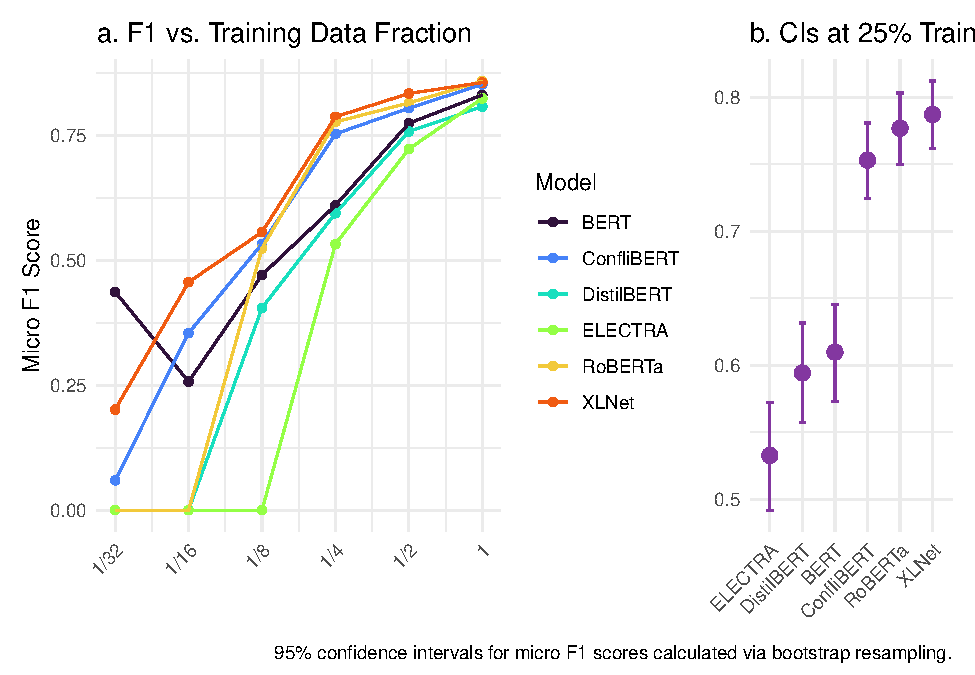
\includegraphics[keepaspectratio]{satp-classification_files/figure-pdf/target_type_performance-1.pdf}}

}

\caption{Model Performance for `Target Type' Task}

\end{figure}%

At full training (Figure 4a, rightmost points), model scores converge
somewhat, but still lag those observed in the action type task.
ConfliBERT reaches 0.878, with RoBERTa (0.870) and XLNet (0.869) close
behind. However, performance tails off for BERT (0.847), DistilBERT
(0.826), and ELECTRA (0.787). These figures indicate that target
prediction is a more difficult task overall, likely due to higher class
imbalance and greater semantic ambiguity in the expression of target
entities.

\begin{figure}[H]

{\centering \pandocbounded{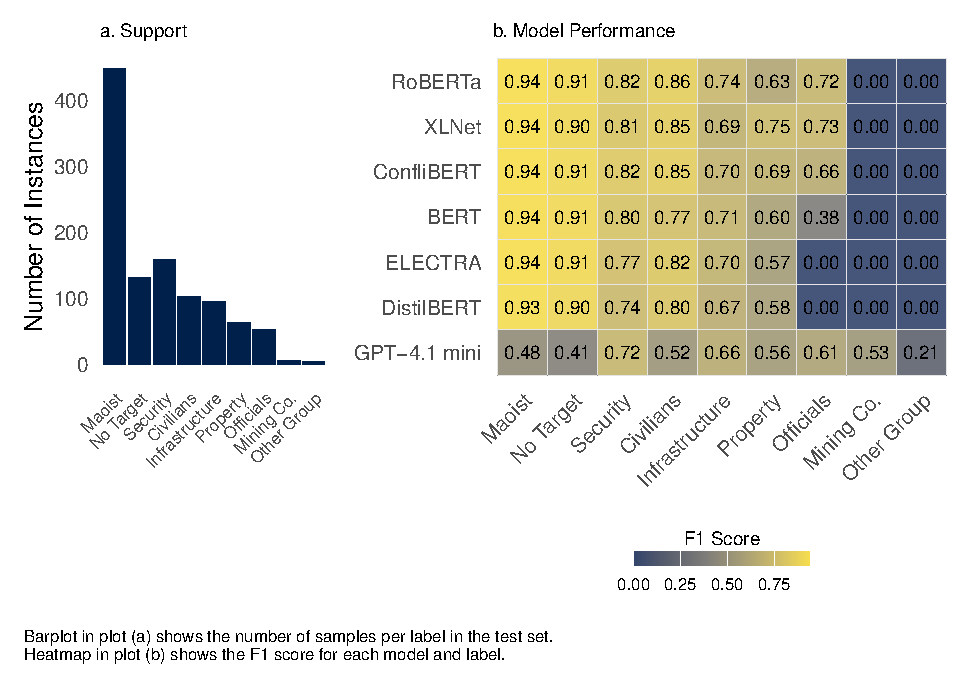
\includegraphics[keepaspectratio]{satp-classification_files/figure-pdf/target_type_labels-1.pdf}}

}

\caption{Model Performance and Test Set Support by `Target Type' Label}

\end{figure}%

Figure 5 further illustrates this point by breaking down F1 scores
across individual labels. Some target types---particularly those with
limited support in the training set---show markedly lower performance.
However, the decline is not solely attributable to frequency. For
example, Surrender in the action task achieved strong scores despite low
support, likely due to its lexical distinctiveness. By contrast,
Infrastructure/Facility targets underperform even when relatively
frequent, suggesting that greater lexical variability and ambiguity in
how these targets are described contributes to model error.

\subsection{Performance-Speed
Tradeoffs}\label{performance-speed-tradeoffs}

Figure 6 presents a performance--speed comparison for the action and
target type classification tasks, plotting micro F1 scores against
evaluation speed (measured in samples per second). The figure highlights
the trade-offs between model accuracy and runtime efficiency, which are
especially relevant for researchers working in low-resource or
latency-sensitive environments.

\begin{figure}[H]

{\centering \pandocbounded{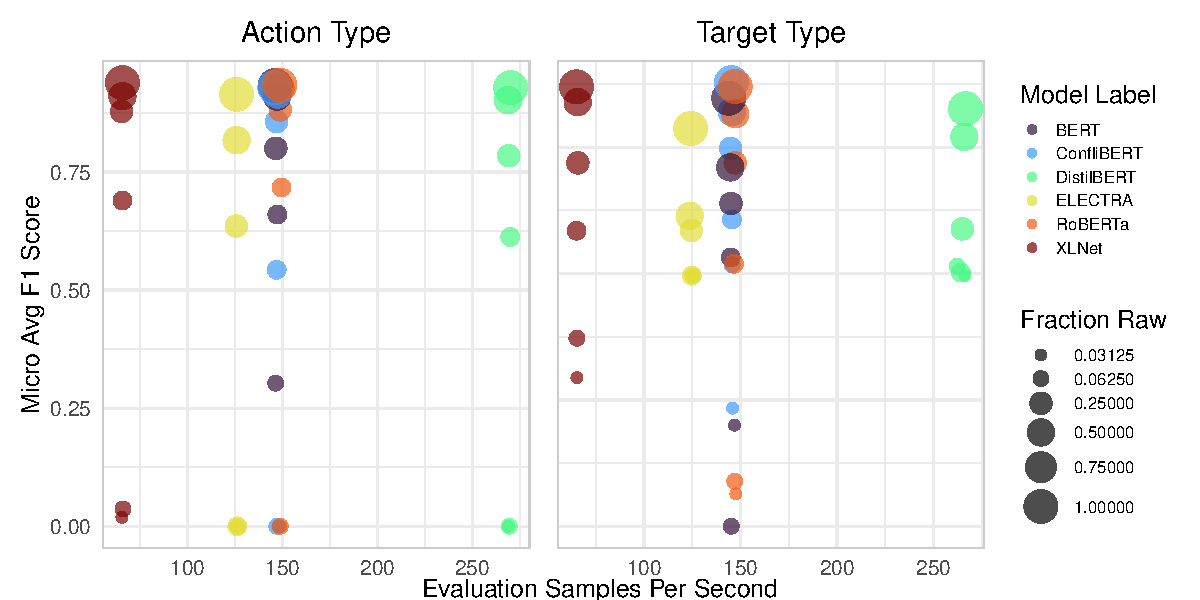
\includegraphics[keepaspectratio]{satp-classification_files/figure-pdf/performance_vs_speed-1.pdf}}

}

\caption{Model Performance vs.~Speed for Multiclass Classification
Tasks}

\end{figure}%

Among the top-performing models, RoBERTa and ConfliBERT stand out for
their efficiency. At full training, both achieve micro F1 scores near
the top of the range---0.870 and 0.878, respectively (on the target
task)---while maintaining high evaluation speeds of 147 and 145 samples
per second. BERT, while slightly less performant (0.847), operates at a
comparable speed (144 samples/sec), making it a viable option where
pretraining data diversity is sufficient.

In contrast, XLNet, though highly competitive in terms of accuracy
(0.869), is much slower, evaluating at only 65 samples per second---less
than half the speed of RoBERTa and ConfliBERT. This substantial
performance-cost trade-off limits XLNet's practical appeal in
time-constrained settings.

DistilBERT emerges as the fastest model, running at 267 samples per
second, but as seen earlier, it tends to underperform at lower training
fractions, making it less suitable for small-data scenarios. ELECTRA
performs poorly on both axes: it is the least accurate model (0.787) and
also slower than most of its peers (124 samples/sec), suggesting limited
utility for either high-accuracy or speed-critical tasks.

Though Figure 6 focuses on the action and target type tasks, patterns
are similar for the perpetrator classification task (not shown). In all
cases, the results suggest that RoBERTa and ConfliBERT offer the best
balance between accuracy and efficiency, particularly when high
throughput is required alongside strong classification performance.

\section{Conclusion}\label{conclusion}

This study evaluated the performance of large language models (LLMs) on
a multi-label classification task using a subset of hand-coded events
from the South Asia Terrorism Portal (SATP) covering the Maoist
insurgency in India. The dataset reflects the type of bespoke coding
often found in social science research, where events are labeled across
multiple dimensions with a custom taxonomy developed for a specific
analytical purpose.

Our analysis showed that LLMs performed reasonably well on
high-frequency labels, particularly when those labels were lexically
distinctive or closely tied to surface-level textual features. For
instance, labels like killing and arrest were predicted with relatively
high accuracy even with limited training data. As the volume of training
data increased, model performance improved overall, but the gains were
not evenly distributed across labels.

Performance on low-frequency labels remained limited, with models often
failing to predict these categories reliably. Some labels, such as
infrastructure attacks, saw improvements with more training data, but
still lagged behind more common categories. We also observed that
multi-label performance varied by model and training fraction,
suggesting that LLMs are sensitive to both model capacity and data
availability in these settings.

These findings indicate that LLMs can serve as effective tools for
assisting with annotation on certain types of labels---especially those
that are frequent and lexically grounded---but remain less reliable for
rare or semantically diffuse labels. In practice, this means that LLMs
could potentially reduce the human labor required for annotating
well-represented event types, while human oversight is still needed for
more challenging cases.

Future work should explore strategies for improving performance on the
tail of the label distribution. One possibility is oversampling rare
labels during training to mitigate class imbalance. Another is data
augmentation, including paraphrasing or targeted generation of examples
for underrepresented categories. More structured approaches, such as
organizing labels hierarchically or embedding them in a continuous
space, may also help models generalize across related labels.

In addition, further analysis of model errors could inform refinements
to both the coding scheme and the annotation process. For example,
identifying which labels are frequently confused may help clarify
category definitions or guide the construction of auxiliary tasks to
sharpen model distinctions.

Finally, while this study focused on a single dataset, the challenges it
raises are broadly relevant to social scientists considering the use of
LLMs for classification tasks. Bespoke annotation schemes and imbalanced
label distributions are common features of applied research, and this
work contributes initial guidance on where LLMs are likely to be useful
and where further development is needed. The SATP dataset provides a
valuable testbed for continued experimentation with these methods.

\section*{References}\label{references}
\addcontentsline{toc}{section}{References}

\phantomsection\label{refs}
\begin{CSLReferences}{1}{0}
\bibitem[\citeproctext]{ref-brandt2024}
Brandt, Patrick T., Sultan Alsarra, Vito J. D`Orazio, Dagmar Heintze,
Latifur Khan, Shreyas Meher, Javier Osorio, and Marcus Sianan. 2024.
{``{ConfliBERT}: {A Language Model} for {Political Conflict}.''}
December 19, 2024. \url{https://doi.org/10.48550/arXiv.2412.15060}.

\bibitem[\citeproctext]{ref-clark2020}
Clark, Kevin, Minh-Thang Luong, Quoc V. Le, and Christopher D. Manning.
2020. {``{ELECTRA}: {Pre-training Text Encoders} as {Discriminators
Rather Than Generators}.''} March 23, 2020.
\url{https://doi.org/10.48550/arXiv.2003.10555}.

\bibitem[\citeproctext]{ref-devlin2019}
Devlin, Jacob, Ming-Wei Chang, Kenton Lee, and Kristina Toutanova. 2019.
{``{BERT}: {Pre-training} of {Deep Bidirectional Transformers} for
{Language Understanding}.''} May 24, 2019.
\url{https://doi.org/10.48550/arXiv.1810.04805}.

\bibitem[\citeproctext]{ref-halterman2023}
Halterman, Andrew, Philip A. Schrodt, Andreas Beger, Benjamin E.
Bagozzi, and Grace I. Scarborough. 2023. {``Creating {Custom Event Data
Without Dictionaries}: {A Bag-of-Tricks}.''} April 3, 2023.
\url{https://doi.org/10.48550/arXiv.2304.01331}.

\bibitem[\citeproctext]{ref-heseltine2024}
Heseltine, Michael, and Bernhard Clemm von Hohenberg. 2024. {``Large
Language Models as a Substitute for Human Experts in Annotating
Political Text.''} \emph{Research \& Politics} 11 (1):
20531680241236239. \url{https://doi.org/10.1177/20531680241236239}.

\bibitem[\citeproctext]{ref-hu2022}
Hu, Yibo, MohammadSaleh Hosseini, Erick Skorupa Parolin, Javier Osorio,
Latifur Khan, Patrick Brandt, and Vito D'Orazio. 2022. {``{ConfliBERT}:
{A Pre-trained Language Model} for {Political Conflict} and
{Violence}.''} In \emph{Proceedings of the 2022 {Conference} of the
{North American Chapter} of the {Association} for {Computational
Linguistics}: {Human Language Technologies}}, 5469--82. Seattle, United
States: Association for Computational Linguistics.
\url{https://doi.org/10.18653/v1/2022.naacl-main.400}.

\bibitem[\citeproctext]{ref-liu2019}
Liu, Yinhan, Myle Ott, Naman Goyal, Jingfei Du, Mandar Joshi, Danqi
Chen, Omer Levy, Mike Lewis, Luke Zettlemoyer, and Veselin Stoyanov.
2019. {``{RoBERTa}: {A Robustly Optimized BERT Pretraining Approach}.''}
July 26, 2019. \url{https://doi.org/10.48550/arXiv.1907.11692}.

\bibitem[\citeproctext]{ref-ornstein2023}
Ornstein, Joseph T, Elise N Blasingame, and Jake S Truscott. 2023.
{``How to {Train Your Stochastic Parrot}: {Large Language Models} for
{Political Texts}.''}

\bibitem[\citeproctext]{ref-osorio2024}
Osorio, Javier, Sultan Alsarra, Amber Converse, Afraa Alshammari, Dagmar
Heintze, Latifur Khan, Naif Alatrush, et al. 2024. {``Keep It {Local}:
{Comparing Domain-Specific LLMs} in {Native} and {Machine Translated
Text} Using {Parallel Corpora} on {Political Conflict}.''} In \emph{2024
2nd {International Conference} on {Foundation} and {Large Language
Models} ({FLLM})}, 542--52. Dubai, United Arab Emirates: IEEE.
\url{https://doi.org/10.1109/FLLM63129.2024.10852489}.

\bibitem[\citeproctext]{ref-sanh2020}
Sanh, Victor, Lysandre Debut, Julien Chaumond, and Thomas Wolf. 2020.
{``{DistilBERT}, a Distilled Version of {BERT}: Smaller, Faster, Cheaper
and Lighter.''} March 1, 2020.
\url{https://doi.org/10.48550/arXiv.1910.01108}.

\bibitem[\citeproctext]{ref-yang2020}
Yang, Zhilin, Zihang Dai, Yiming Yang, Jaime Carbonell, Ruslan
Salakhutdinov, and Quoc V. Le. 2020. {``{XLNet}: {Generalized
Autoregressive Pretraining} for {Language Understanding}.''} January 2,
2020. \url{https://doi.org/10.48550/arXiv.1906.08237}.

\end{CSLReferences}




\end{document}
